\documentclass[10pt,a4paper,twocolumn]{article}
\usepackage[english]{babel}
\usepackage[utf8]{inputenc}
\usepackage[plainpages=false,pdfpagelabels,unicode]{hyperref}
\usepackage[pdftex]{graphicx}
\usepackage[margin=1.5cm, includefoot]{geometry}
\usepackage{authblk}
\usepackage[numbers,sort&compress]{natbib}
\usepackage{mhchem}

\author[a,b,c]{Pavel Ondračka}
\author[c]{David Holec}
\author[a,b]{Lenka Zajíčková}
\affil[a]{Faculty of Science, Masaryk University, Kotlářská 2, 611 37 Brno, Czech Republic}
\affil[b]{CEITEC - Central European Institute of Technology, Masaryk University, Kotlářská 2, 611 37 Brno, Czech Republic}
\affil[c]{Department of Physical Metallurgy and Materials Testing, Montanuniversität Leoben, Franz-Josef-Straße 18, Leoben A-8700, Austria}

\title{Optical properties of monoclinic, cubic, tetragonal and amorphous HfO$_2$ with TB-mBJ}
\date{}

\begin{document}

\twocolumn[
  \begin{@twocolumnfalse}
    \maketitle
    \begin{abstract}

    \end{abstract}
  \end{@twocolumnfalse}
]

\section{Introduction}
HfO$_2$ is attracting a lot of attention as a high-$k$ material for electronic applications~\cite{Houssa2006, Robertson2006} as well as optical applications such as antireflective coatings~\cite{Fadel1998, Khoshman2008}, heat-mirrors~\cite{Al-Kuhaili2004}, or laser mirrors~\cite{Meng2012}).

HfO$_2$ can exist in several polymorphs, depending on growth conditions.
There are three low presure polymorphs of HfO$_2$, monoclinic (P 1 21/c 1, spacegroup: 14), tetragonal (P 42/n m c, spacegroup: 137) and cubic (F m -3 m, spacegroup: 225), shown in figure \ref{structs}.
Monoclinic phase is stable at ambient conditions, transforms to tetragonal phase at $\sim$1700\,$^\circ$C and later to cubic phase at $\sim$2600\,$^\circ$C. %FIXME: some citation.

\begin{figure}[b]
   \begin{center}
   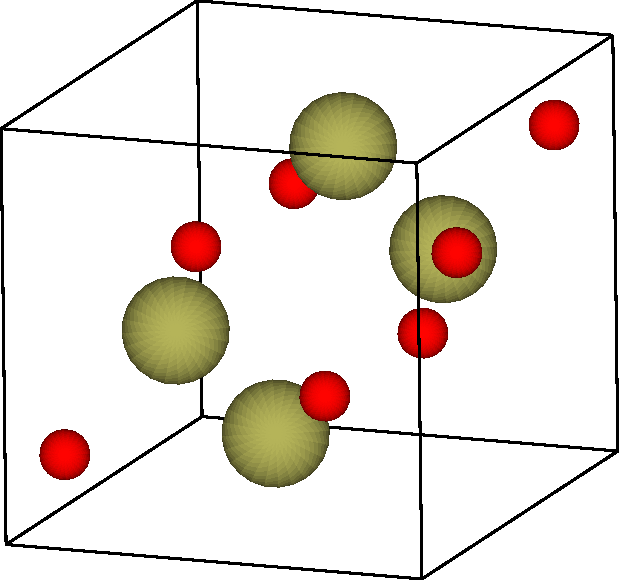
\includegraphics[width=0.3\linewidth]{figures/monoclinic.pdf}
   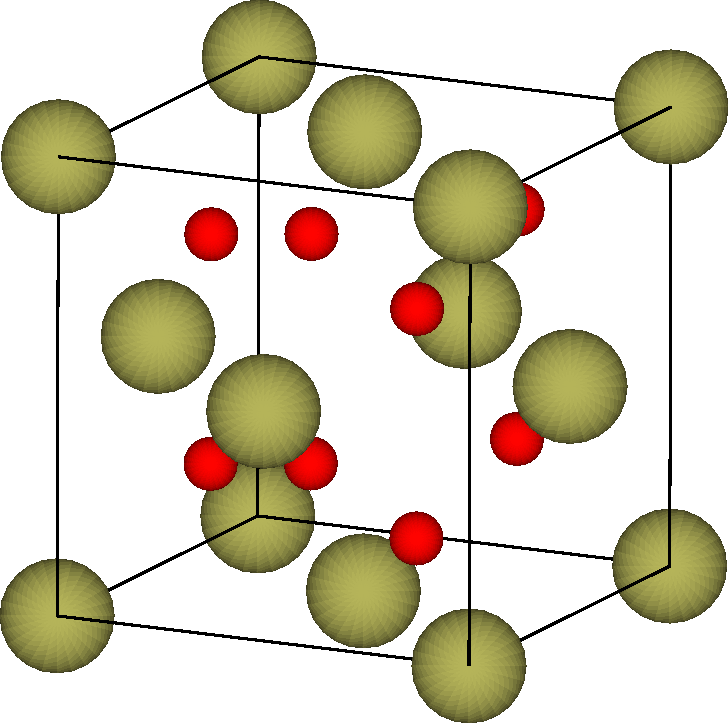
\includegraphics[width=0.3\linewidth]{figures/tetragonal.pdf}
   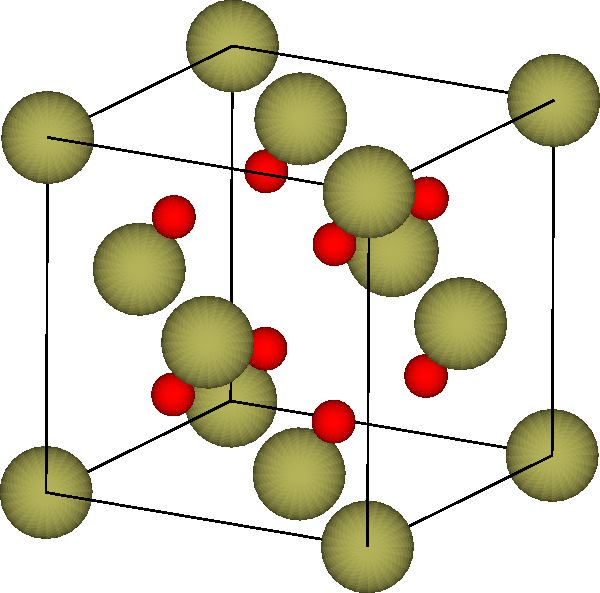
\includegraphics[width=0.3\linewidth]{figures/cubic.pdf}
   \caption{Crystal structure of a) monoclinic, b) tetragonal, and c) cubic hafnia, drawn by VESTA~\cite{Momma2011} }
   \label{structs}
   \end{center}
\end{figure}

Apart from the experimental works, there are numerous \textit{ab initio} studies focused on structural, mechanical, electronic or optical properties of HfO$_2$ \cite{Caravaca2005, Broqvist2007, Ceresoli2006, Garcia2004, Kaneta2007, Liu2009, Scopel2008, Terki2008, Zhao2002, Gruning2010}.

However, majority of the HfO$_2$ \textit{ab initio} studies employ conventional approximations for the exchange-correlation (xc) potential, local density approximation (LDA) or generalised gradient approximation (GGA).
One shortcoming, of those approximations is the well known underestimation for the band gap.

%Since well calculated band gap and band structure is critical for correct prediction of optical properties.

On the other hand, hybrid functionals or other more sophisticated methods as GW, give band gaps in much better agreement with experiment, however are much more computationally expansive.
A recently developed semi-local xc potential (modified Becke-Johnson, TB-mBJ) is an alternative that can provide highly accurate band gaps at the computational cost of LDA or GGA~\cite{Tran2009}.

Band gap of monoclinic HfO$_2$ was already found to be 5.83\,eV using the original TB-mBJ parameters~\cite{Koller2012}.
This is in a good agreement with the experimental value of 5.68\,eV \cite{Balog1977}, it is however unclear, if this extends also to other forms of HfO$_2$.
Also the optical properties of HfO$_2$ calculated with TB-mBJ were to our knowledge not yet studied.
%This problem can be seen in case of TiO$_2$, where we have a very good agreement in calculated band gap for anatase, however the difference for calculated and experimental values for rutile is almost twice as big \cite{Sai2012}.

%The huge impact of the improved description of the electronic structure on the predicted optical properties, such as refractive index, $n$, extinction coefficient, $\kappa$, or dielectric function $\epsilon$, when employing the mBJ potential was shown by \citet{Sai2012} for the case of rutile and anatase TiO$_2$.

In this work, we thoroughly test the applicability of TB-mBJ potential for monoclinic, tetragonal, cubic and amorphous HfO$_2$ with focus on band gap and optical properties.

\section{Methodology}

There is no exchange energy functional for TB-mBJ~\cite{Tran2009}, hence its not suitable for structural optimization based on the total energy minimisation.
The initial HfO$_2$ monoclinic, tetragonal and cubic cells were structurally optimized with respect to internal positions and lattice parameters.
This was done using the the Vienna Ab initio Simulation Package~\cite{Kresse1996}, with projector augmented pseudopotentials \cite{Kresse1999} and using the generalised gradient approximation parametrized by Perdew, Burke and Ernzerhof (GGA-PBE) \cite{Perdew1996}.
The number of $k$-points reflected the size of the modelled cell by keeping product (number of $k$-points)$\cdot$(number of atoms) constant and equal to approximatelly 2500.
The plane wave energy cut-off of 500\,eV used for crystalline polymorphs was reduced to 300\,eV for the amorphous models.
Consequently, a total energy accuracy of several meV/atom was achieved.

Amorphous unit cells were prepared by the simulated annealing procedure.
96 atoms were randomly distributed inside a cubic simulation box with a side 10.1503\,\AA{} corresponding to mass density of 10.695\,g/cm$^3$.
An \textit{ab initio} molecular dynamics run at 5000\,K for 3\,ps with a time step of 3\,fs provided a thermally equilibrated distribution of the atoms inside the cell.
In the next step, the cell temperature was decreased to 0\,K in 100 (fast) or 1000 (slow) steps, each corresponding to 3\,fs.
Finally, the resulting models were relaxed with respect to atom positions and cell volume (i.e., mass density).

Electronic and optical properties were calculated for the structurally relaxed models using Wien2k, a full potential all electron code~\cite{Blaha2001} employing the linearized augmented plane wave method.
A dense k-grid of 17$\times$17$\times$16 for monoclinic, 24$\times$24$\times$16 for tetragonal, 27$\times$27$\times$27 for cubic, and 4$\times$4$\times$4 for amorphous was used in order to obtain converged optical properties.
Atomic spheres radii were set to almost matching spheres corresponding to approximately (depending on polymorph) $\sim$1.7\,\AA{} for oxygen and $\sim$1.9\,\AA{} for hafnia.
The $R_{mt} \cdot K_{max}$ matrix size parameter was set to 9, roughly equivalent to 410\,eV cut-off parameter in pseudopotential calculations.

The TB-mBJ with the original parametrisation by \citet{Tran2009} was used for exchange and LDA for the correlation potential. For determination of dielectric functions we used the optic code~\cite{AmbroschDraxl2006}, a part of the Wien2k package, which utilizes Random Phase Approximation (RPA) neglecting local field effects.

A Lorentz broadening of 0.03\,eV was used for the dielectric function for better comparison with room temperature experimental data.

\section{Results a discussion}

\subsection{Structural properties}

\begin{table*}
\begin{center}
\begin{tabular}{ccccccccc}

 & & $a$\,[\AA] & $b$\,[\AA] & $c$\,[\AA] & $\gamma\,[^{\circ}]$ &
$B$\,[GPa] & $E_f$\,[eV/atom] & $\Delta E$\,[eV/atom]\\
m & GGA, present & 5.143 & 5.190 & 5.330 & 99.6 & 197 & -3.975 & 0.000
\\%-10.2026 \\
  & LDA, present & 5.035 & 5.123 & 5.198 & 99.6 & 194 & -4.318 & 0.000
\\%-11.0841 \\
  & exp., \citet{Adam1959} & 5.1156 & 5.1722 & 5.2948 & 99.23 & & & \\

m2 & GGA, present & 5.661 & 5.662 & 5.999 & 117.8 & 183 & -3.972 &
0.003\\ %-10.2005 \\
   & LDA, present & 5.534 & 5.606 & 5.775 & 115.8 & 193 & -4.234 &
0.084\\ %-10.9998 \\

t & GGA, present & 3.591 & & 5.219 & 90 & 175 & -3.920 & 0.055\\ %-10.1483 \\
  & LDA, present & 3.526 & & 5.073 & 90 & 220 & -4.280 & 0.038\\ %-11.0459 \\
  & exp., \citet{Curtis1954} & 5.14 & & 5.25 & & & & \\

c & GGA, present & 5.075 & & & 90.0 & 255 & -3.890 & 0.085 \\%-10.1176 \\
  & LDA, present & 4.982 & & & 90.0 & 289 & -4.261 & 0.057 \\%-11.0274
  & exp., \citet{Senft1983} & 5.110 & & & & & & \\

\end{tabular}
\caption{Overview of calculated structural properties}
\label{structure}
\end{center}
\end{table*}

The four structures considered in the present work (monoclinic, cubic, tetragonal, and amorphous) were fully optimised with respect to the unit cell shape and atom positions at several fixed volumes.
In doing so, we used both GGA and LDA exchange-correlation potentials which typically overestimate and underestimate, respectively, lattice parameters with respect to experimental values.
The thus obtained energy vs. volume data were fitted with Birch-Murnaghan equation of state \cite{Birch1947}.
Resulting lattice parameters are listed in Table \ref{structure} together with the selected experimental and \textit{ab initio} data from literature for comparison.
The energy of formation was calculated as
\begin{equation}
  E_f^\alpha=E_0(\ce{HfO2}^\alpha) - \frac13 (E_0(\ce{Hf}) + E_0(\ce{O2}))\ ,
\end{equation}
where $E_0(\ce{HfO2}^\alpha)$, $E_0(\ce{Hf})$, and $E_0(\ce{O2})$ are the \textit{ab initio} total energies (per atom) of \ce{HfO2} in the $\alpha$ structure (monoclinic, cubic, tetragonal, or amorphous), Hf in the hcp structure, and an oxygen molecule, respectively.

%% FIXME GGA: Hf: -9.8322 eV/at, O -4.42597 eV/at

% &&  $\rho\,[\mathrm{g/cm^3}]$ & $B$\,[GPa] & $E_f$\,[eV/atom] \\
% am & GGA, present & 9.922 & 92 & -3.776 & 0.199\\ %-10.0043

The most stable structure is, in agreement with the equilibrium phase diagram, the monoclinic structure, followed by tetragonal (experimentally high temperature) and cubic structures.
The least stable configuration yielding the highest energy of formation, is the amorphous structure.
The optimised lattice parameters are in good agreement with the previously published data, the GGA values being generally closer to the experimental values.

%% FIXME
The optimisation of the amorphous structure yielded estimates for the equilibrium mass density: $\rho_{\mathrm{GGA}}=10.375\,\mathrm{g/cm^3}$, $\rho_{\mathrm{LDA}}=9.425\,\mathrm{g/cm^3}$. %%FIXME????
This is about the same values as predicted for the tetragonal structures, while the monoclinic and cubic structures are predicted to be slightly less and more dense, respectively.

An interesting phenomena is predicted for the monoclinic variant.
As shown in Fig.\ref{EV}, the energy vs. volume data exhibit a second minimum (quite a shallow one in the LDA case) for volumes larger than the equilibrium (structural parameters are denoted as m2 in Table \ref{structure}).
Consequently, a structural transformation is predicted for isothermal volume expansion.
The most distinct feature is a step-like change of the monoclinic angle gamma from $99.6\deg$ (GGA/LDA) to $117.8\deg$ (GGA) and $115.8\deg$ (LDA) (see insets in Fig.~\ref{EV}).
A similar structural transition has been recently reported for the monoclinic phase in NiTi shape memory alloys \cite{Holec2011-tg}.
There, the structural complexity of this phase resulted in a hysteresis of the forwards and backwards pressure-induced phase transformation.
We envision that a similar phenomena may appear also for the monoclinic \ce{HfO2}.

\begin{figure}
\begin{center}
	\includegraphics[width=\linewidth]{figures/m-EV.pdf}
	\caption{E-V and $\gamma$ data for the monoclinic structure calculated with GGA-PBE and LDA. Lines are fits of the Birch-Murnaghan equation of state around the minima (only the highlighted points were fitted).}
   \label{EV}
\end{center}
\end{figure}

\subsection{Band gaps}

\begin{table*}
\begin{center}

\begin{tabular}{c|ccccc}
			& TB-mBJ & PBE & hybrid funkcionals & GW$_0$ & experiment \\
\hline
m-HfO$_2$ &	5.76 & 4.08 & PBE0: 6.75~\cite{Komsa2010}, HSE06: 5.98~\cite{Komsa2010} & 5.9~\cite{Gruning2010} & 5.68~\cite{Balog1977} \\
c-HfO$_2$ &	5.88 & 3.77 & SX: 5.6~\cite{Clark2010}, HSE06: 5.38~\cite{Yang2014} & 5.5~\cite{Gruning2010} & 5.8$^A$~\cite{Lim2002}\\
t-HfO$_2$ &	6.54 & 4.79 &  & 6.0~\cite{Gruning2010} & \\
am-HfO$_2$ & 5.53, 5.65 & & PBE0: 5.3~\cite{Broqvist2007}, 5.94~\cite{Chen2011} &  & 5.49--5.72~\cite{Takeuchi2004}, 5.62~\cite{Nguyen2005}, 5.7~\cite{Perevalov2007}\\

\end{tabular}
\caption{Overview of calculated band gaps compared to experiment and other \textit{ab initio} calculations}
\label{gaps}
\end{center}
\end{table*}

Table \ref{gaps} shows overview of calculated band gaps for different HfO$_2$ forms.
Those are compared to experiment and to band gaps calculated by other \textit{ab initio} methods.
For m-HfO$_2$ we have obtained a calculated band gap of of 5.76\,eV.
This is a perfect agreement with experimental value of 5.68\,eV~\cite{Balog1977} and comparable to HSE06 hybrid (5.98\,eV)~\cite{Komsa2010} and 5.9\,eV obtained by GW$_0$~\cite{Gruning2010}.
It is also in better agreement with experiment than PBE0 hybrid functional (6.75\,eV)~\cite{Komsa2010}.

Calculated band gap of c-HfO$_2$ has a value of 5.88\,eV.
This seems to be a slight overestimation in comparison to hybrid functionals (SX: 5.6\,eV~\cite{Clark2010}, HSE06: 5.38\,eV~\cite{Yang2014}) and to GW$_0$ (5.5\,eV)~\cite{Gruning2010}.
It is observed, that while for PBE calculations the band gap for c-HfO$_2$ is 0.3\,eV lower that for m-HfO$_2$, with TB-mBJ it is 0.1\,eV higher.
Comparison to experiment is complicated, as cubic hafnia is not stable at room temperatures and hence it is usually stabilized by yttrium.
For (Y$_2$O$_3$)$_{15}$--(HfO$_2$)$_{85}$ the band gap is 5.8\,eV~\cite{Lim2002}, again comparable to our results.

TB-mBJ band gap for t-HfO$_2$ is 6.54\,eV, highest of all the hafnium polymorphs.
This is in agreement with the GW$_0$ calculation, where the band gap value of 6.0\,eV is also higher than band gap of monoclinic and cubic form, albeit the difference is lower.

%% FIXME add relevant references; explain a bit what is Urbach tail and Tauc plot
While for crystalline hafnia polymorphs the optical band gap was determined directly from the calculations, for amorphous cells another approach was chosen.
This was needed in order to discount the effect of Urbach tail, defect states and to facilitate better comparison with experimental data obtained by means of Tauc plot.
Optical band gap in amorphous cells was thus obtained by fitting linear part of square root of the joint density of states and extrapolating to zero.

FIXME: show both the optical gap from "tauc fit" and the electronic gap for amorphous cells, maybe show the JDOS fits?

Calculated optical band gap for amorphous hafnia is 5.65\,eV, again in good agreement with experimental values ranging from 5.49\,eV to 5.72\,eV~\cite{Takeuchi2004, Nguyen2005, Perevalov2007}.

FIXME: update gap and optical constants for both am1 and am2 structures when calculations finish.

All calculated band gaps are significantly improved in comparison to PBE values of 4.08, 3.77, and 4.79\,eV for monoclinic, cubic and tetragonal HfO2 respectively.

\subsection{Optical properties}

Calculated optical properties are shown in figures \ref{eps-cHfO2}, \ref{eps-tHfO2}, \ref{eps-mHfO2}, \ref{eps-amHfO2}.
One independent component of the dielectric tensor was calculated for cubic, two for tetragonal and four for monoclinic hafnia.
Three diagonal components were calculated for amorphous hafnia, however they were found to be almost identical, thus confirming the cell amorphousness.
The dielectric tensor is oriented such that the xx component is parallel to the $a$ axis, yy lies in the plane defined by $a$ and $b$ axes, perpendicular to xx, and zz is perpendicular to xx and yy components.

Experimental dielectric functions for m-HfO$_2$ by \citet{Edwards2003} and \citet{Nguyen2005} are included for comparison.
It is clearly visible, that calculated imaginary part of the dielectric function is underestimated in comparison to experiment.
The other distinctive feature in the experimental data which we fail to reproduce is the peak at 6\,eV, however according to \cite{Takeuchi2004} it is caused by oxygen vacancies and hence its absence in calculations is expected.
No experimental data are available for tetragonal hafnia.
Similar problem appears when comparing calculated optical properties for cubic and amorphous HfO$_2$ to those of \citet{Lim2002} and \citet{Nguyen2005} respectively.

To understand better the reason for shift of the absorption to higher energies in comparison to the experimental data, we have compared the calculated dielectric function for m-HfO$_2$ with hybrid based calculations using the Yukawa screened PBE0 functional (YS-PBE0) \cite{Tran2011} and we observed similar shift of the dielectric function maximum.
Hence we believe that this discrepancy is not caused by incorrectly calculated band structure, but rather by the random phase approximation used during calculation of the dielectric function.

FIXME: show the real part or only the imaginary? Maybe some discussion about electronic part of static dielectric constant.

\begin{figure}
\begin{center}
	\includegraphics[width=\linewidth]{figures/c-HfO2.pdf}
	\caption{Calculated dielectric function of c-HfO$_2$}
   \label{eps-cHfO2}
\end{center}
\end{figure}

\begin{figure}
\begin{center}
	\includegraphics[width=\linewidth]{figures/t-HfO2.pdf}
	\caption{Calculated dielectric function of t-HfO$_2$}
   \label{eps-tHfO2}
\end{center}
\end{figure}

\begin{figure}
\begin{center}
	\includegraphics[width=\linewidth]{figures/m-HfO2.pdf}
	\caption{Calculated dielectric function of m-HfO$_2$}
   \label{eps-mHfO2}
\end{center}
\end{figure}

\begin{figure}
\begin{center}
	\includegraphics[width=\linewidth]{figures/am-HfO2.pdf}
	\caption{Calculated dielectric function of am-HfO$_2$}
   \label{eps-amHfO2}
\end{center}
\end{figure}


\section{Conclusions}

It was shown, that

\section*{Acknowledgments}
This work was supported by the IT4Innovations Centre of Excellence project (CZ.1.05/1.1.00/02.0070), funded by the European Regional Development Fund and the national budget of the Czech Republic via the Research and Development for Innovations Operational Programme, as well as Czech Ministry of Education, Youth and Sports via the project Large Research, Development and Innovations Infrastructures (LM2011033).

\bibliographystyle{unsrtnat}
\bibliography{bib-db}

\end{document}
